\question
Булева функция задана диаграммой Эйлера-Венна. Представьте эту функцию в письменном виде, обязательно используя элементы XOR, NAND, NOR, и изобразите в виде схемы функциональных отношений.

\begin{figure}[h]

\begin{minipage}[h]{0.55\linewidth}
\end{minipage}
\begin{minipage}[h]{0.45\linewidth}
\center{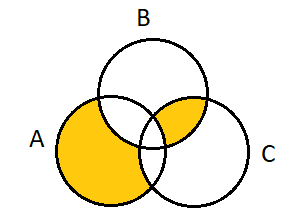
\includegraphics[width=0.7\textwidth]{pic/881.png} }
\end{minipage}
\end{figure}

---------------

Автор -- Марат Ибрагимов, М3219